\begin{enumerate}
	\item If $\tan \brak{\frac{x+y}{x-y}}=k$,then $\dfrac{dy}{dx}$ is equal to 

			\item $\frac{-y}{x}$
   \item $\frac{y}{x}$
			
			\item $\sec^{2}\brak{\frac{y}{x}}$ 
   \item $-\sec^{2}\brak{\frac{y}{x}}$ 
			
  \item  \textbf{Assertion(A) :}Maximum value of $\brak{{\cos^{-1}}}^2$ is ${{\pi}^2}$.\\
  \textbf{Reason(R):}Range of the principle value branch of ${{\cos^{-1}x}}$ is $\sbrak{{\frac{\pi}{2}},{\frac{\pi}{2}}}$.
	\item If $y=\sqrt{ax+b}$ , prove that $y\brak{\dfrac{d^2y}{dx^2}}+\brak{\dfrac{dy}{dx}}^2=0$ 
 \item If the circumference of circle is increasing at the constant rate, prove that rate of change of area of circle is directly proportional to its radius.

 \item Engine displacement is the measure of the cylinder volume swept by all the pistons of a piston engine.The piston moves inside the cylinder bore  
  \begin{figure}[H]
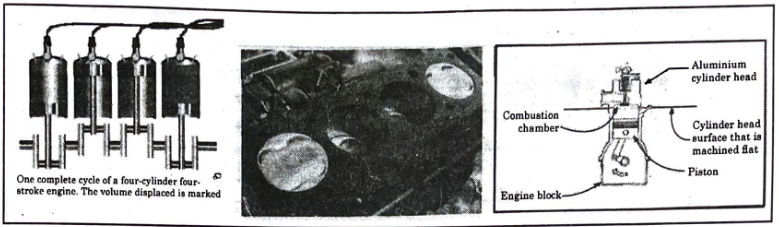
\includegraphics[width=\columnwidth]{figs/engine.png}
\caption{}
\label{fig:engine}
\end{figure}
 %use figure environment for inserting figure   

 \item The cylinder bore in the form of circular cylinder open at the top is to be made from a metal sheet of area ${75\pi}$ ${cm}^2.$ \\
Based on the above information , answer the following questions: 

 \begin{enumerate}[label=(\roman*)]

     \item  If the radius of cylinder is r cm and height is h cm, then write the volume V of cylinder in terms of radius r. 
     \item Find $\dfrac{dv}{dr}$ 
     
     \item 
	     \begin{enumerate}[label=(\alph*)]
     \item Find the radius of cylinder when its volume is maximum. 
   
     \item  For maximum volume, $h > r$.State true or false and justify. 
 \end{enumerate}
 \end{enumerate}

 \item The use of electric vehicles will curb air pollution in the long run.
 
\begin{figure}[H]
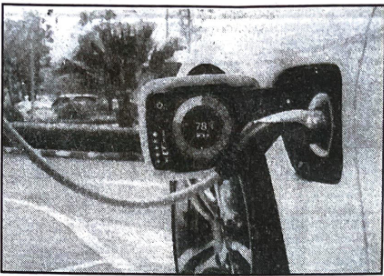
\includegraphics[width=\columnwidth]{figs/electricvehicle.png}
\caption{}
\label{fig:electricvehicle}
\end{figure}
  
 \item The use of electric vehicles is increasing every year and estimated electric vehicles in use at any time $t$ is given by the function $V$ :
 
 \begin{align}
    V\brak{t}=\frac{1}{5}t^3 - \frac{5}{2}t^2 + 25t-2 
 \end{align}
 Where $t$ represents the time and $t$=1,2,3\dots corresponds to year 2001,2002,2003\dots respectively.\\
 Based on the above information, answer the following questions :
 \begin{enumerate}[label=(\roman*)]
     \item Can the above function be used to estimate number of vehicles in the year 2000 ? Justify. 
     \item Prove that the function V\brak{t} is an increasing function.
 \end{enumerate}

\item The slope of the normal to the curve $y=2x^2+3\sin{x}$ at $x=0$ is \rule{30pt}{1pt}.

\item The total revenue (in \rupee) received from sale of x units of a product is $R(x)$ = $3x^2+36x+5$. The marginal revenue, when $x=12$ is \rule{30pt}{1pt}.

\item If $\sin y = x \sin(a+y)$, then prove that $\frac {dy}{dx} = \frac {\sin x^2(a+y)}{\sin a}$.

\item Find the equation of tangent to the curve $y=x^2+4x+1$ at the point(3,22).

\item If $Y = \tan^{-1}\left(\frac{3x - x^3}{1 - 3x^2}\right)$,-$\frac{1}{\sqrt{3}}$ \textless x \textless $\frac{1}{\sqrt{3}}$
then find $\frac{dy}{dx}$ and $\frac{{d^2y}}{{dx^2}}$.

\item If $\sec^{-1}\left(\frac{1+x}{1-y}\right)=a$, then $\frac{dy}{dx}$ is equal to

\item The oder and degree of the differential equation of the family of parabolas having at 
organ and axis along positive x-axis is

\item If $y = \log x$, then $\frac{{d^2y}}{{dx^2}}$=

\item Find the intervals in which the function f defined as $f(x) = \sin(x) + \cos(x)$,
$0 \leq x \leq 2\pi$ is strictly increasing or decreasing.

\item Prove that the radius of the right circular 
cylindar of greatest curved surface area which 
can be inscribed in a given cone is half of thatof the cone.

\item If $y=x^{\sin x }+\sin^{-1}(\sqrt x )$, the find $\frac{dy}{dx}$.

\item The supply function of a commodity is 
$100p = (x+20)^2$. Find the Producer's
Surplus(PS),whne the market price is \rupee 25.

\item Find:
$\int{\frac{2x^2 + 1}{x^2 - 3x + 2}}$dx

 \end{enumerate}
